\documentclass[english,11pt]{beamer}

\DeclareMathOperator{\Cov}{Cov}
\DeclareMathOperator{\Var}{Var}
\DeclareMathOperator{\E}{\mathbb{E}}
\DeclareMathOperator{\Proba}{\mathbb{P}}

\newcommand{\Covb}[2]{\ensuremath{\Cov\!\left[#1,#2\right]}}
\newcommand{\Eb}[1]{\ensuremath{\E\!\left[#1\right]}}
\newcommand{\Pb}[1]{\ensuremath{\Proba\!\left[#1\right]}}
\newcommand{\Varb}[1]{\ensuremath{\Var\!\left[#1\right]}}

% norm
\newcommand{\norm}[1]{\| #1 \|}

\newcommand{\indep}{\rotatebox[origin=c]{90}{$\models$}}





\usepackage{mathptmx,amsmath,amssymb,graphicx,bibentry,bbm,babel,ragged2e}

\makeatletter

\newcommand{\noun}[1]{\textsc{#1}}
\newcommand{\jitem}[1]{\item \begin{justify} #1 \end{justify} \vfill{}}
\newcommand{\sframe}[2]{\frame{\frametitle{#1} #2}}

\newenvironment{centercolumns}{\begin{columns}[c]}{\end{columns}}
%\newenvironment{jitem}{\begin{justify}\begin{itemize}}{\end{itemize}\end{justify}}

\usetheme{Warsaw}
\setbeamertemplate{footline}[text line]{}
\setbeamercolor{structure}{fg=purple!50!blue, bg=purple!50!blue}

\setbeamersize{text margin left=15pt,text margin right=15pt}

\setbeamercovered{transparent}


\@ifundefined{showcaptionsetup}{}{%
 \PassOptionsToPackage{caption=false}{subfig}}
\usepackage{subfig}

\usepackage[utf8]{inputenc}
\usepackage[T1]{fontenc}



\makeatother

\begin{document}


\title{Models of growth for system of cities : Back to the simple}

\author{J.~Raimbault$^{1,2}$\\
\texttt{juste.raimbault@parisgeo.cnrs.fr}
}


\institute{$^{1}$UMR CNRS 8504 G{\'e}ographie-cit{\'e}s\\
$^{2}$UMR-T IFSTTAR 9403 LVMT\\
}


\date{CCS 2016 - Amsterdam\\\smallskip
\textit{Session Urban 3}\\\smallskip 22th September 2016
}

\frame{\maketitle}





%%%%%%%%%%%%%%%%%%%
%% ABSTRACT

%Understanding growth patterns in complex systems of cities through modeling is an intensive branch of quantitative geography. Complex agent-based models have been recently provided promising results by multi- modeling and intensive computation for pattern discovery and calibration. However simple interaction-based extensions of seminal models of growth (such as the Gibrat model) have not yet been tested and calibrated against real datasets.
%We propose a spatial model of urban growth extending the Gibrat model by adding the contributions of gravity-based interactions to expected growth rates. Moments derivation for the stochastic model allows to implement a deterministic version on expectancies. Working with the Pumain-INED harmonized database for French cities (population of urban areas for 1831-1999), the 4-parameter interaction model is calibrated through intensive computation on grid, using the OpenMole software, yielding e.g. the characteristic interaction distance at different periods. We then add a second order term aimed at integrating interactions between physical transportation networks and cities, through a feedback of physical flows on traversed cities.It allows to obtain better fits and reproduce stylized facts such as hierarchy inversions and apparition of the “tunnel effect” with the development of railway network. We furthermore introduce a novel method to assess the impact of adding parameters to a simulation model on the effectively gained information, as an extension of Akaike Information Criterion to simulation models. This empirical AIC is estimated by comparing AICs for statistical models, with same parameter number, fitting best behavior space obtained by exploration. It confirms that our extension provide a gain of information on the French city system.
%This contribution provides a renewing insight on simple models of urban growth for system of cities, that proves to have good explicative potentialities. It also introduce a methodology to tackle the open question of quantifying overfitting in simulation models.








%%%%%%%%%%%%%%%%%
\section{Introduction}
%%%%%%%%%%%%%%%%%



\sframe{Modeling Urban Growth}{

\textit{Growth in Urban Systems : multi-scalar, heterogeneous drivers, bifurcations and path-dependancy}

\bigskip

\centering

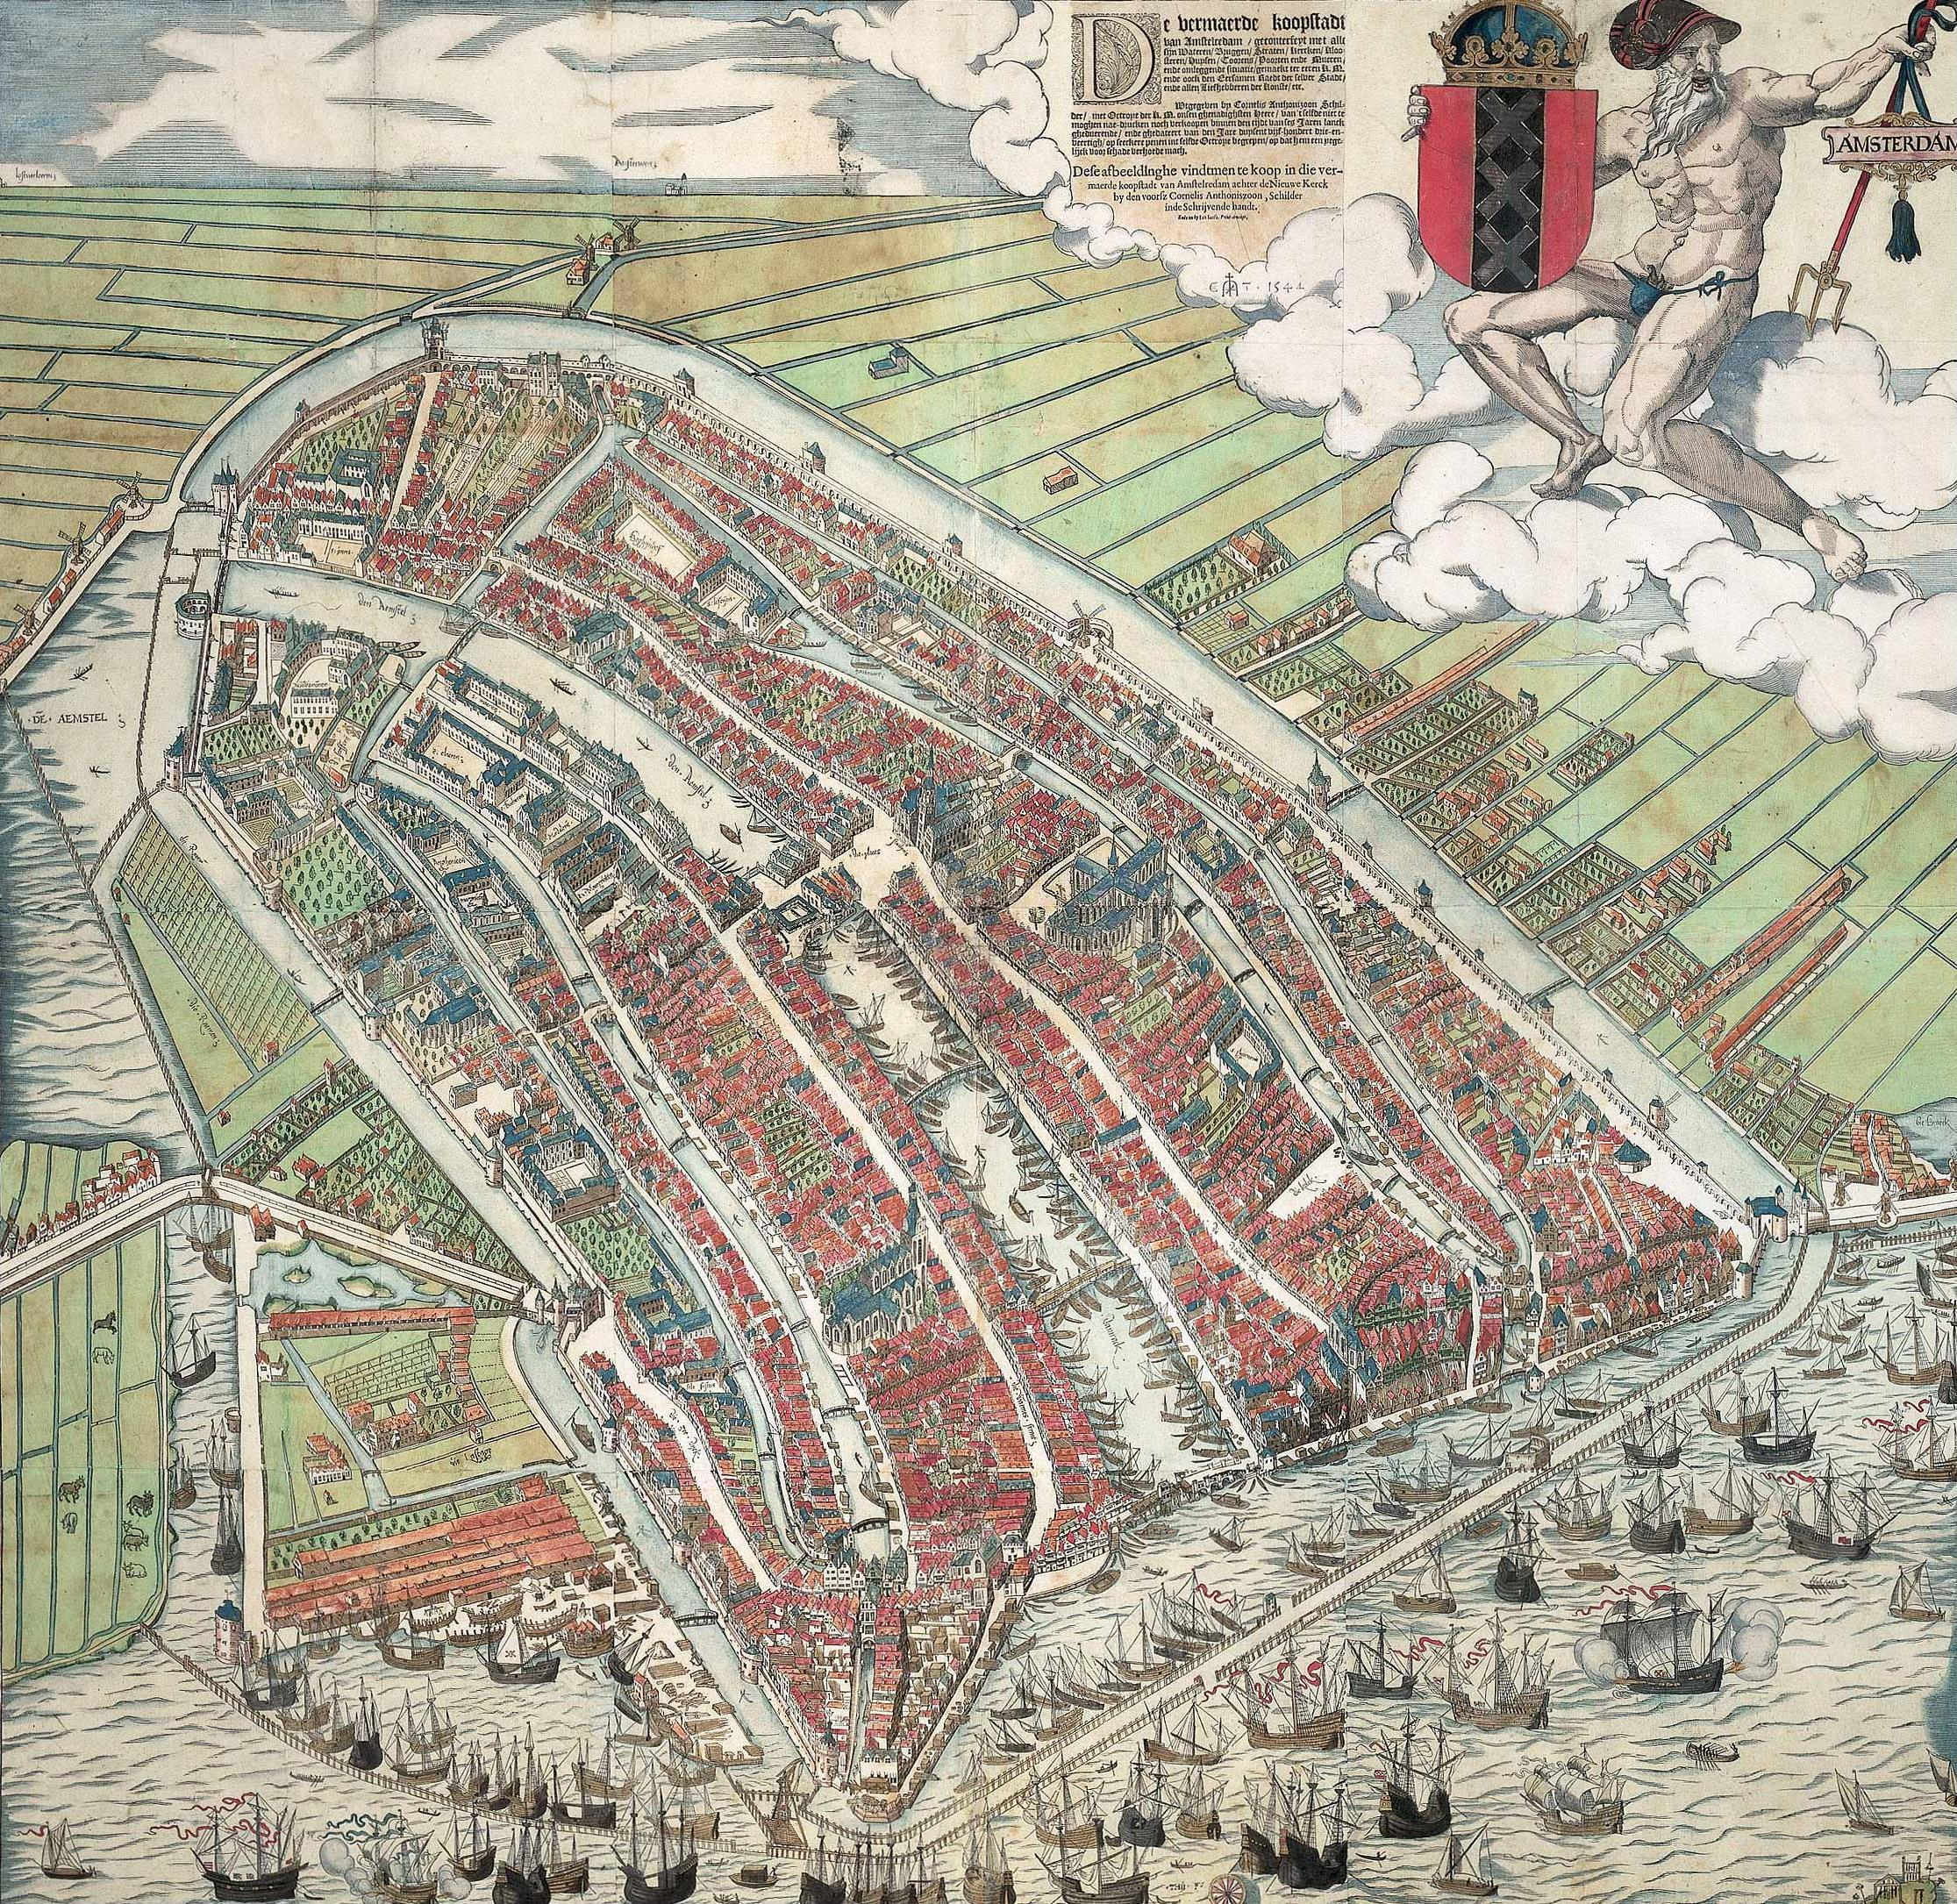
\includegraphics[width=0.45\textwidth,height=0.6\textheight]{figures/Dam1544}
\hspace{0.1cm}
\includegraphics[width=0.45\textwidth,height=0.6\textheight]{figures/Dam1770}

{\tiny Source : Wikipedia}

}

\sframe{Spatial Interaction and Urban Growth}{

\justify

% simpops, extended Gibrat etc

\textit{Role of spatial interactions in Urban Growth ?}

\bigskip
\bigskip

$\rightarrow$ gravity-based flows influence population growth in a synergetic formulation~\cite{sanders1992systeme}

\medskip

$\rightarrow$ Simpop models (from Simpop1 to SimpopLocal) \cite{pumain2012multi} : agent-based approaches ; more recently Marius~\cite{cottineau2015incremental} closer to system dynamics

\medskip

$\rightarrow$ Simple random growth (Gibrat model) becomes quickly complex by adding spatial interaction~\cite{bretagnolle2000long} ; refined extension with waves of innovation in \cite{favaro2011gibrat} 

}


\sframe{Research Objective}{

\justify

$\rightarrow$ \textit{Between complex ABM and non-geographical models in economics/physics, what place for simple models of growth in Urban Systems ?}

\medskip

$\rightarrow$ \textit{Modulation of simple mechanisms to check for necessity/sufficiency : multi-modeling in models of simulation}

\bigskip
\bigskip


\textbf{Research Objective : } Extend Gibrat simple model of growth in system of cities with spatial interactions and feedbacks through physical networks ; Explore systematically and calibrate such families of models


}




%%%%%%%%%%%%%%%%%
\section{Methods and Results}
%%%%%%%%%%%%%%%%%



\sframe{Model Rationale}{

\justify

% bit of theory

\textbf{Rationale :} extend an interaction model for system of cities by including physical network as an additional carrier of spatial interactions (see \cite{raimbault2016memoire} for developed theoretical context) 

\bigskip

$\rightarrow$ Work under Gibrat independence assumptions, i.e. $\Covb{P_i(t)}{P_j(t)}=0$. If $\vec{P}(t+1)=\mathbf{R}\cdot \vec{P}(t)$ where $\mathbf{R}$ is also independent, then $\Eb{\vec{P}(t+1)}=\Eb{\mathbf{R}}\cdot\Eb{\vec{P}}(t)$. Consider expectancies only (higher moments computable similarly)

\medskip

$\rightarrow$ With $\vec{\mu}(t)=\Eb{\vec{P}(t)}$, we generalize this approach by taking $\vec{\mu}(t+1)=f(\vec{\mu}(t))$


}


\sframe{Model Formulation}{

Let $\vec{\mu}(t)=\Eb{\vec{P}(t)}$ cities population and $(d_{ij})$ distance matrix


\medskip

Model specified by

\[
f(\vec{\mu}) = r_0\cdot \mathbf{Id}\cdot \vec{\mu} + \mathbf{G}\cdot \mathbf{1} + \mathbf{N}
\]

 with 
\begin{itemize}
\item $G_{ij} = w_G\cdot \frac{V_{ij}}{<V_{ij}>}$ and $V_{ij} = \left(\frac{\mu_i\mu_j}{\sum{\mu_k}^2}\right)^{\gamma_G} \exp{(-d_{ij}/d_G)}$
\item $N_{i} = w_N \cdot \sum_{kl} \left(\frac{\mu_k\mu_l}{\sum\mu}\right)^{\gamma_N}\exp{(-d_{kl,i})/d_N}$ where $d_{kl,i}$ is distance to shortest path between $k,l$ computed with slope impedance ($Z=\left(1+\alpha/\alpha_0\right)^{n_0}$ with $\alpha_0\simeq 3$)
\end{itemize}



}



\sframe{Data : stylized facts}{


Population data for French-cities (Pumain-INED database : 1831-1999)

% correlation curves, non-stationarity of network effects

\medskip

\textit{Non-stationarity of log-returns correlations function of distance}

\centering

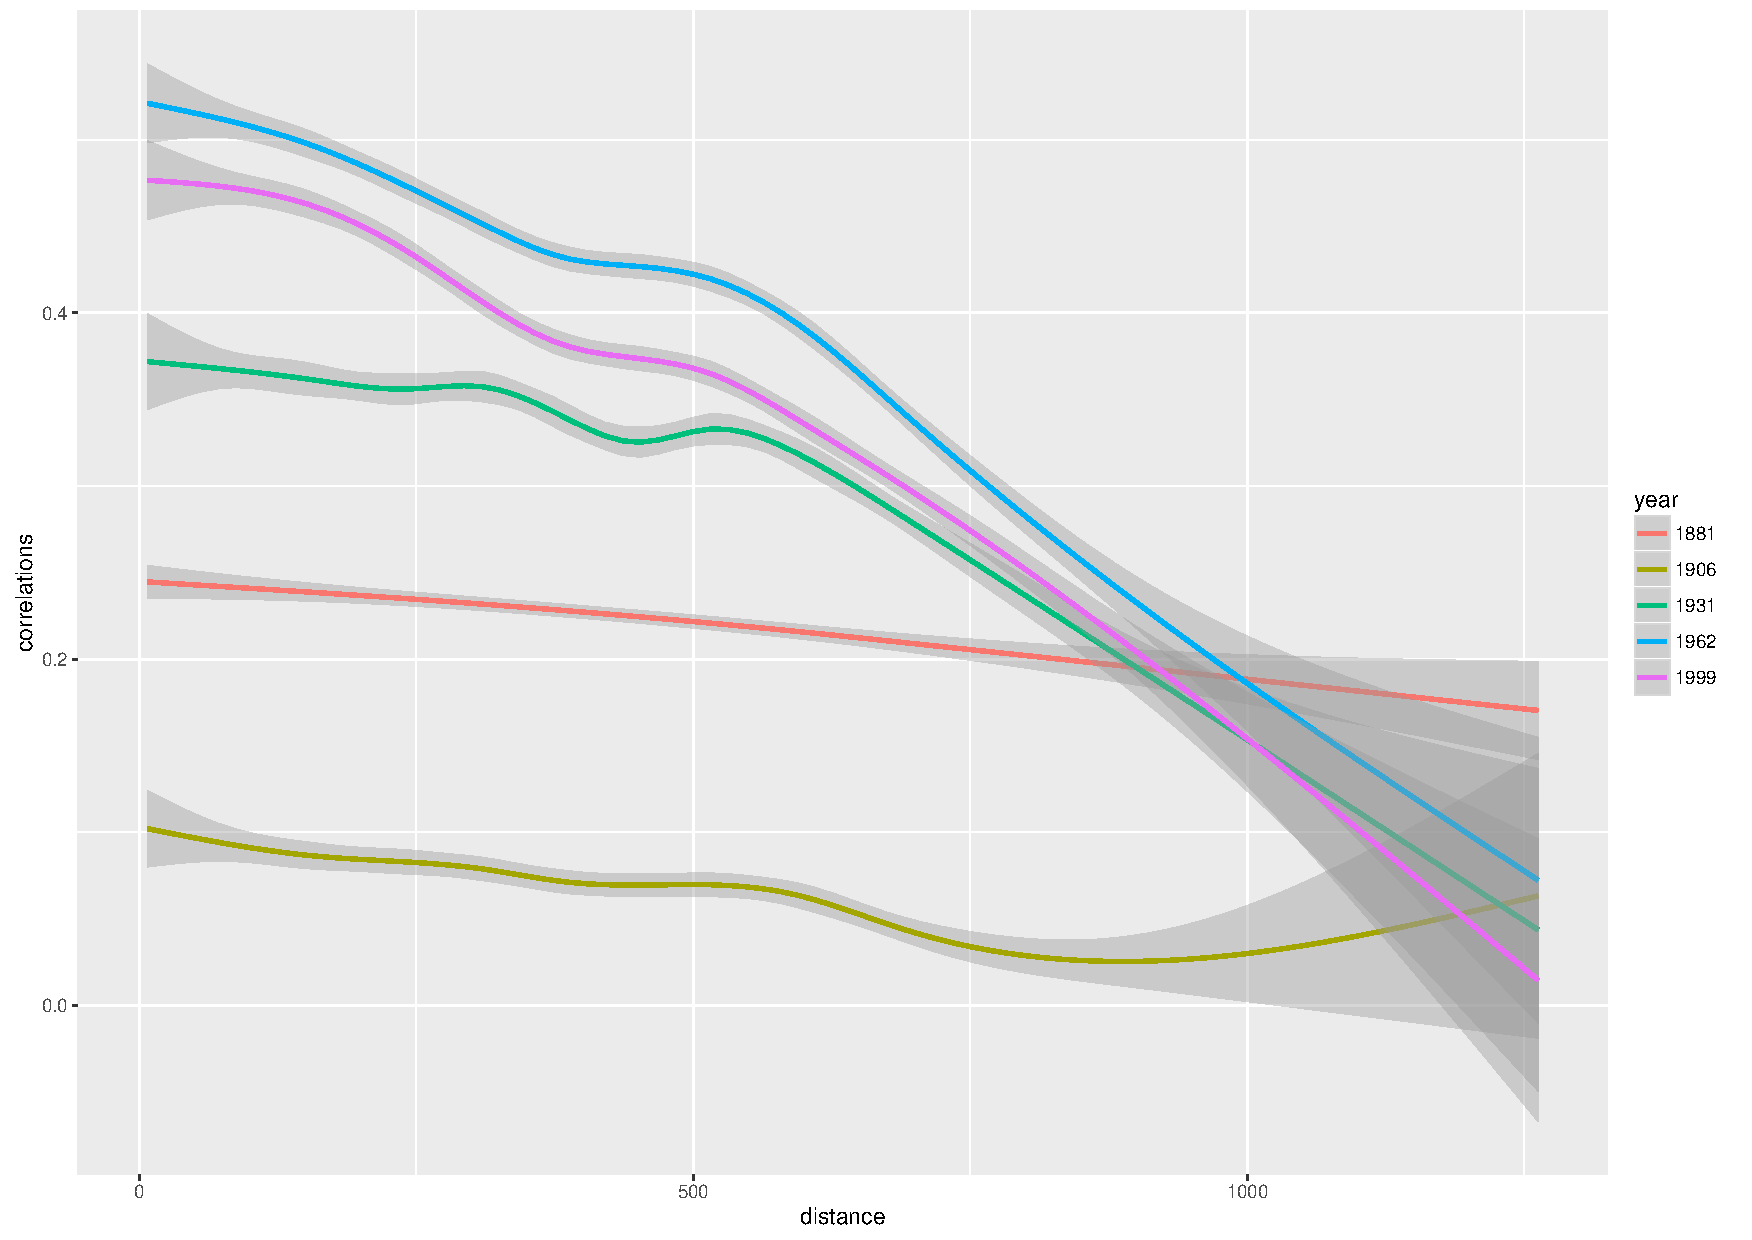
\includegraphics[width=0.8\textwidth,height=0.7\textheight]{figures/empirical_tsCorrelations}

}


\sframe{Data : geographic abstract network}{

% computation of geo shortest paths

\textit{Physical transportation network abstracted through a geographical shortest path network}

% map with shortest path examples

\medskip

\centering

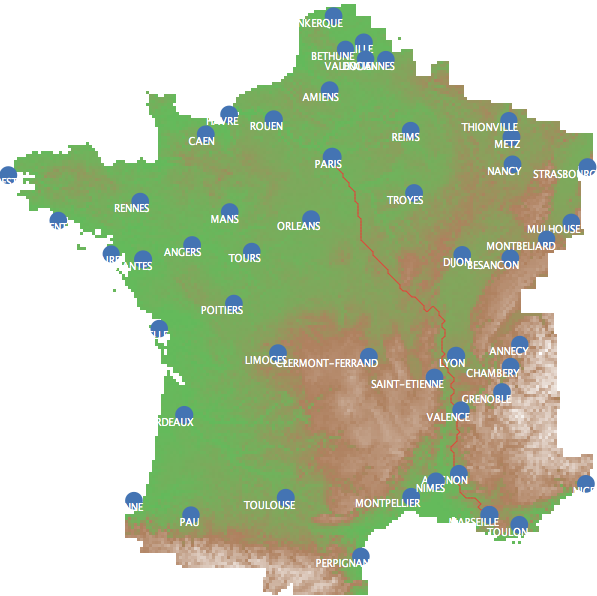
\includegraphics[height=0.75\textheight]{figures/example_shortest_path}

}



\sframe{Implementation}{

\textit{On the importance of visualization in spatial models : complementary implementations in NetLogo/R/Scala}

\medskip

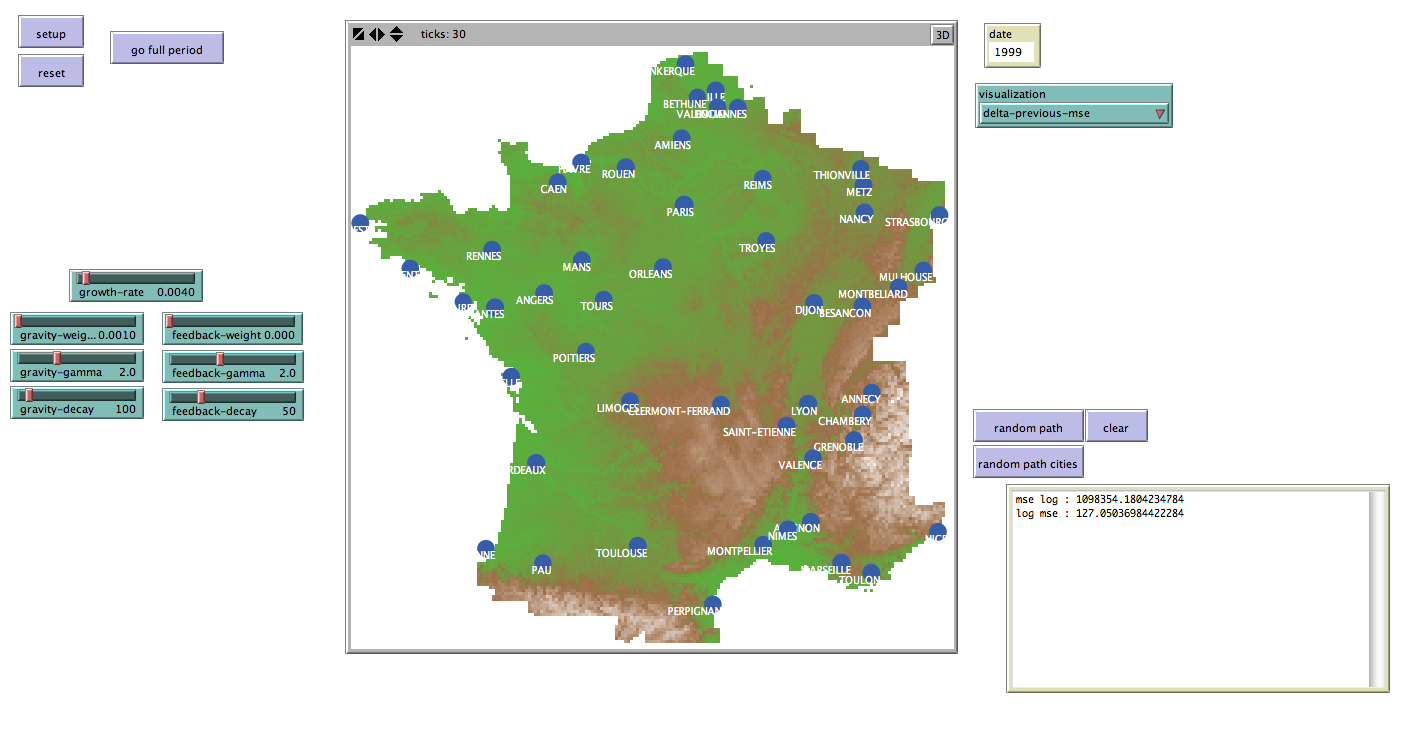
\includegraphics[width=\textwidth]{figures/example_interface}

}



\sframe{Results : model exploration}{

% network effects graphs


\textit{Evidence of physical network effects : fit improve through feedback at fixed gravity}

\medskip

\centering

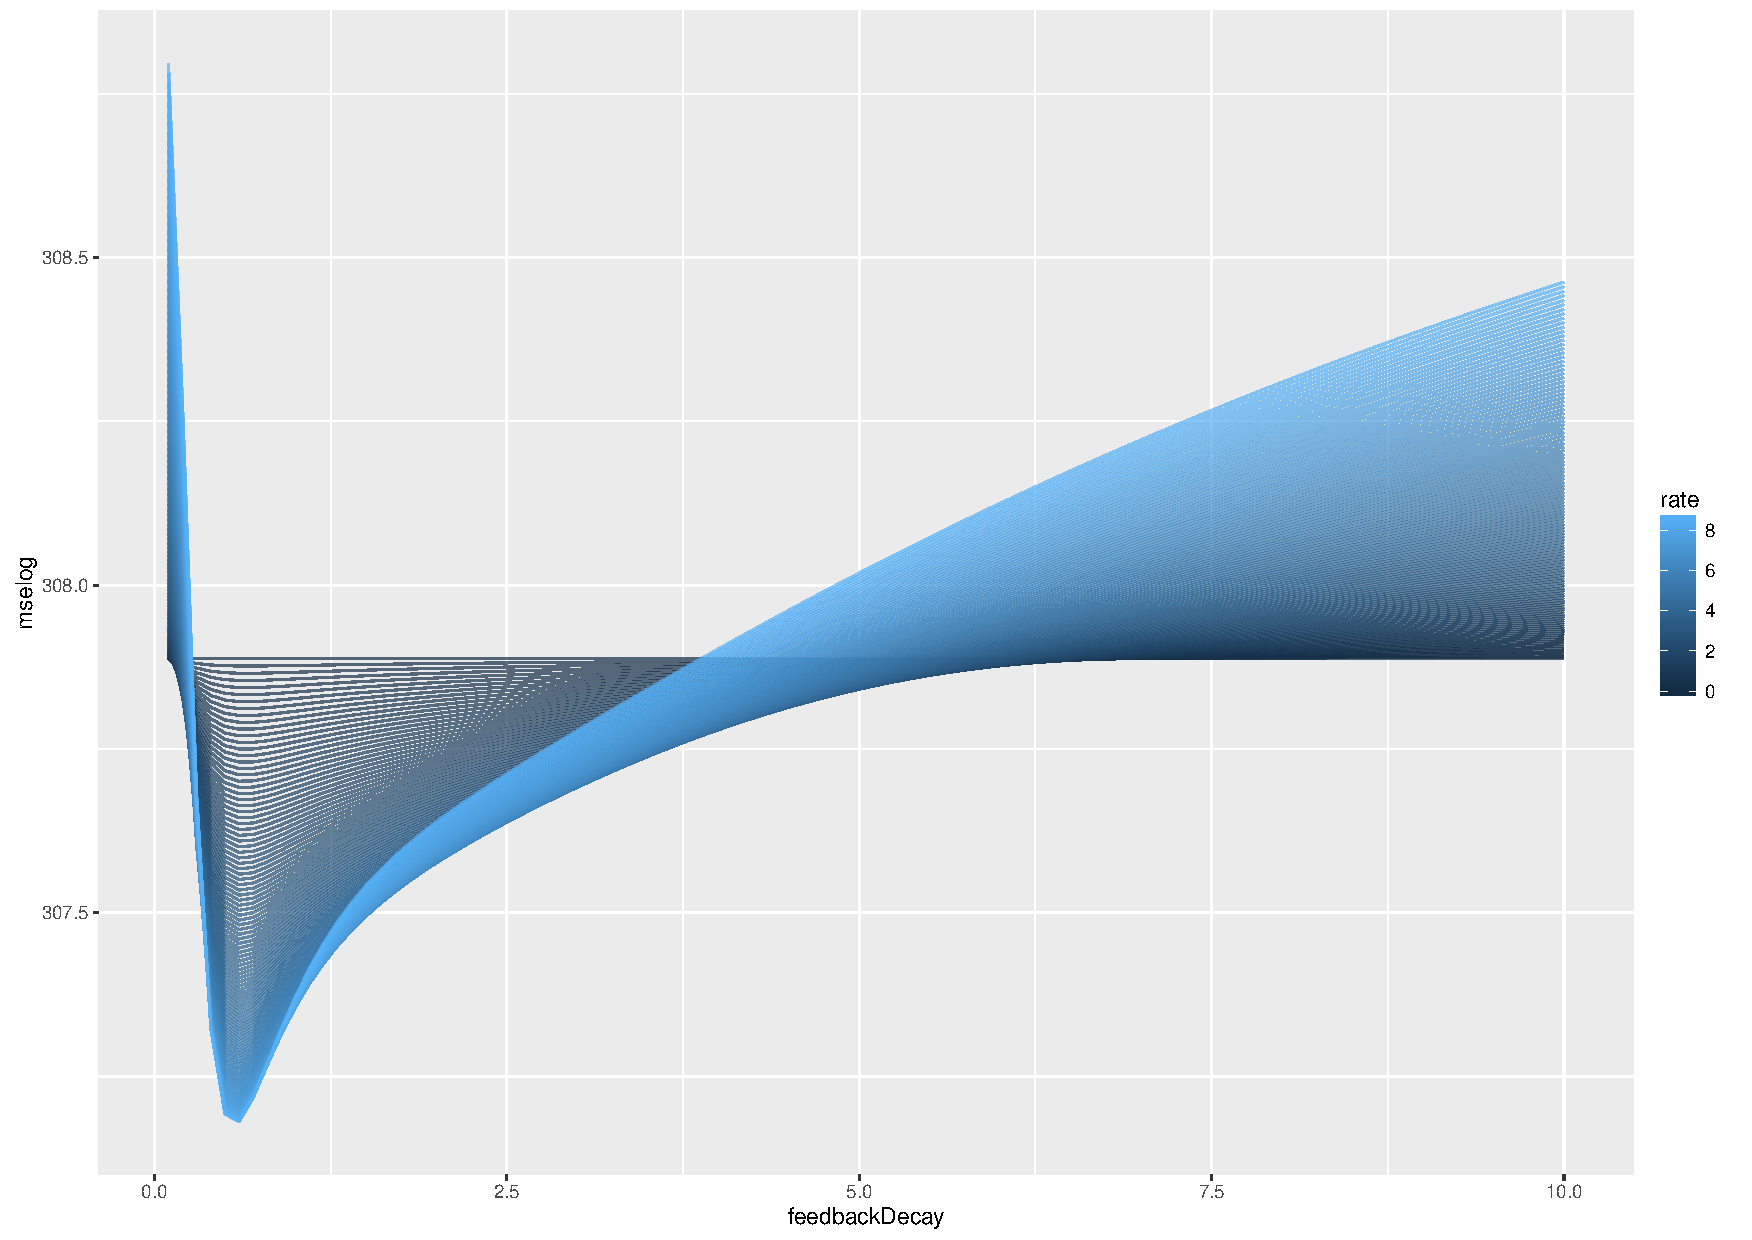
\includegraphics[width=0.8\textwidth,height=0.7\textheight]{figures/mselog-feedbackDecay_ZOOM_fixedgravity}

}

\sframe{Results : model calibration}{

% ga calibration, both full model and gravity only

Model calibration using GA on computation grid, with software \texttt{OpenMole}~\cite{reuillon2013openmole}

\bigskip

\textit{Pareto front for full model calibration, objectives MSE and MSE on logs}

\medskip

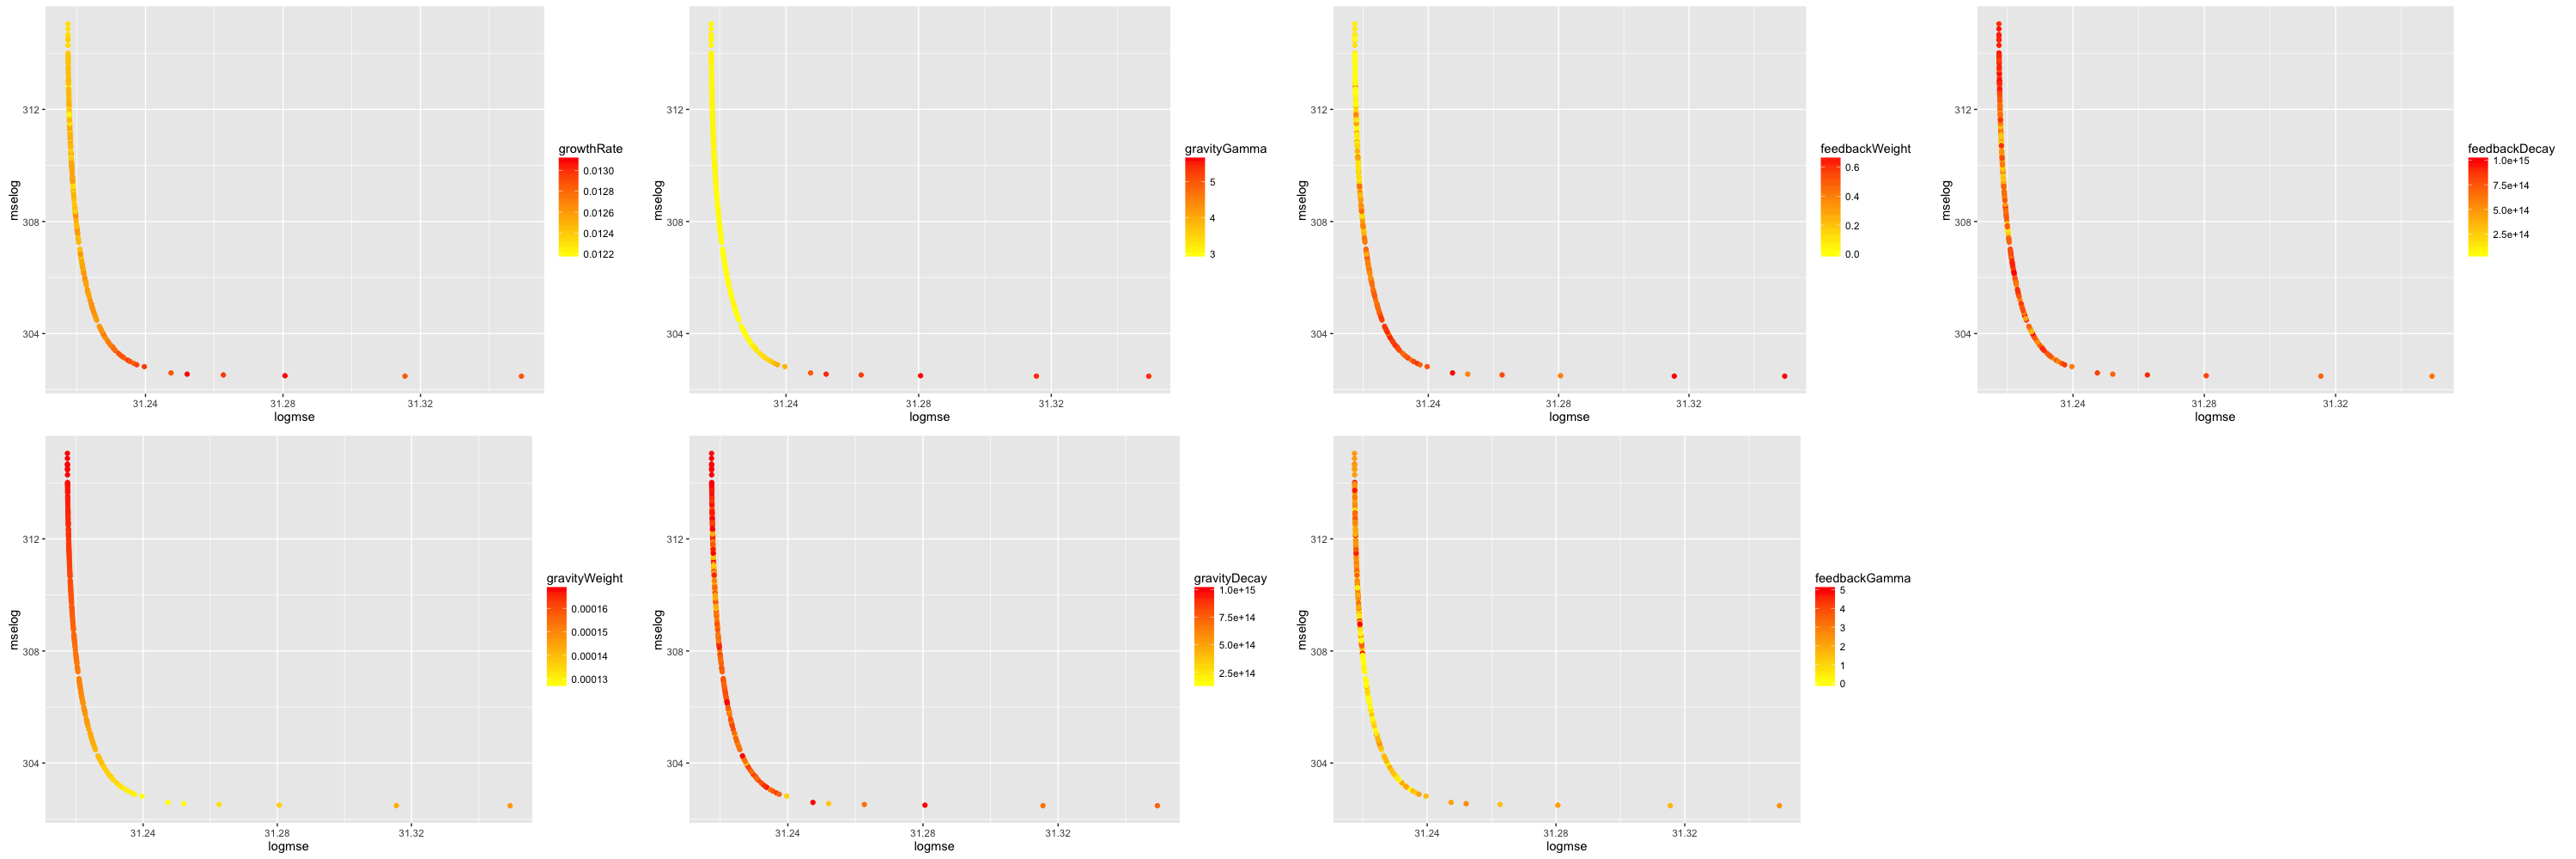
\includegraphics[width=\textwidth,height=0.65\textheight]{figures/pareto_fullmodel}

}




\sframe{Results : non-stationary model calibration}{

% calibration on periods


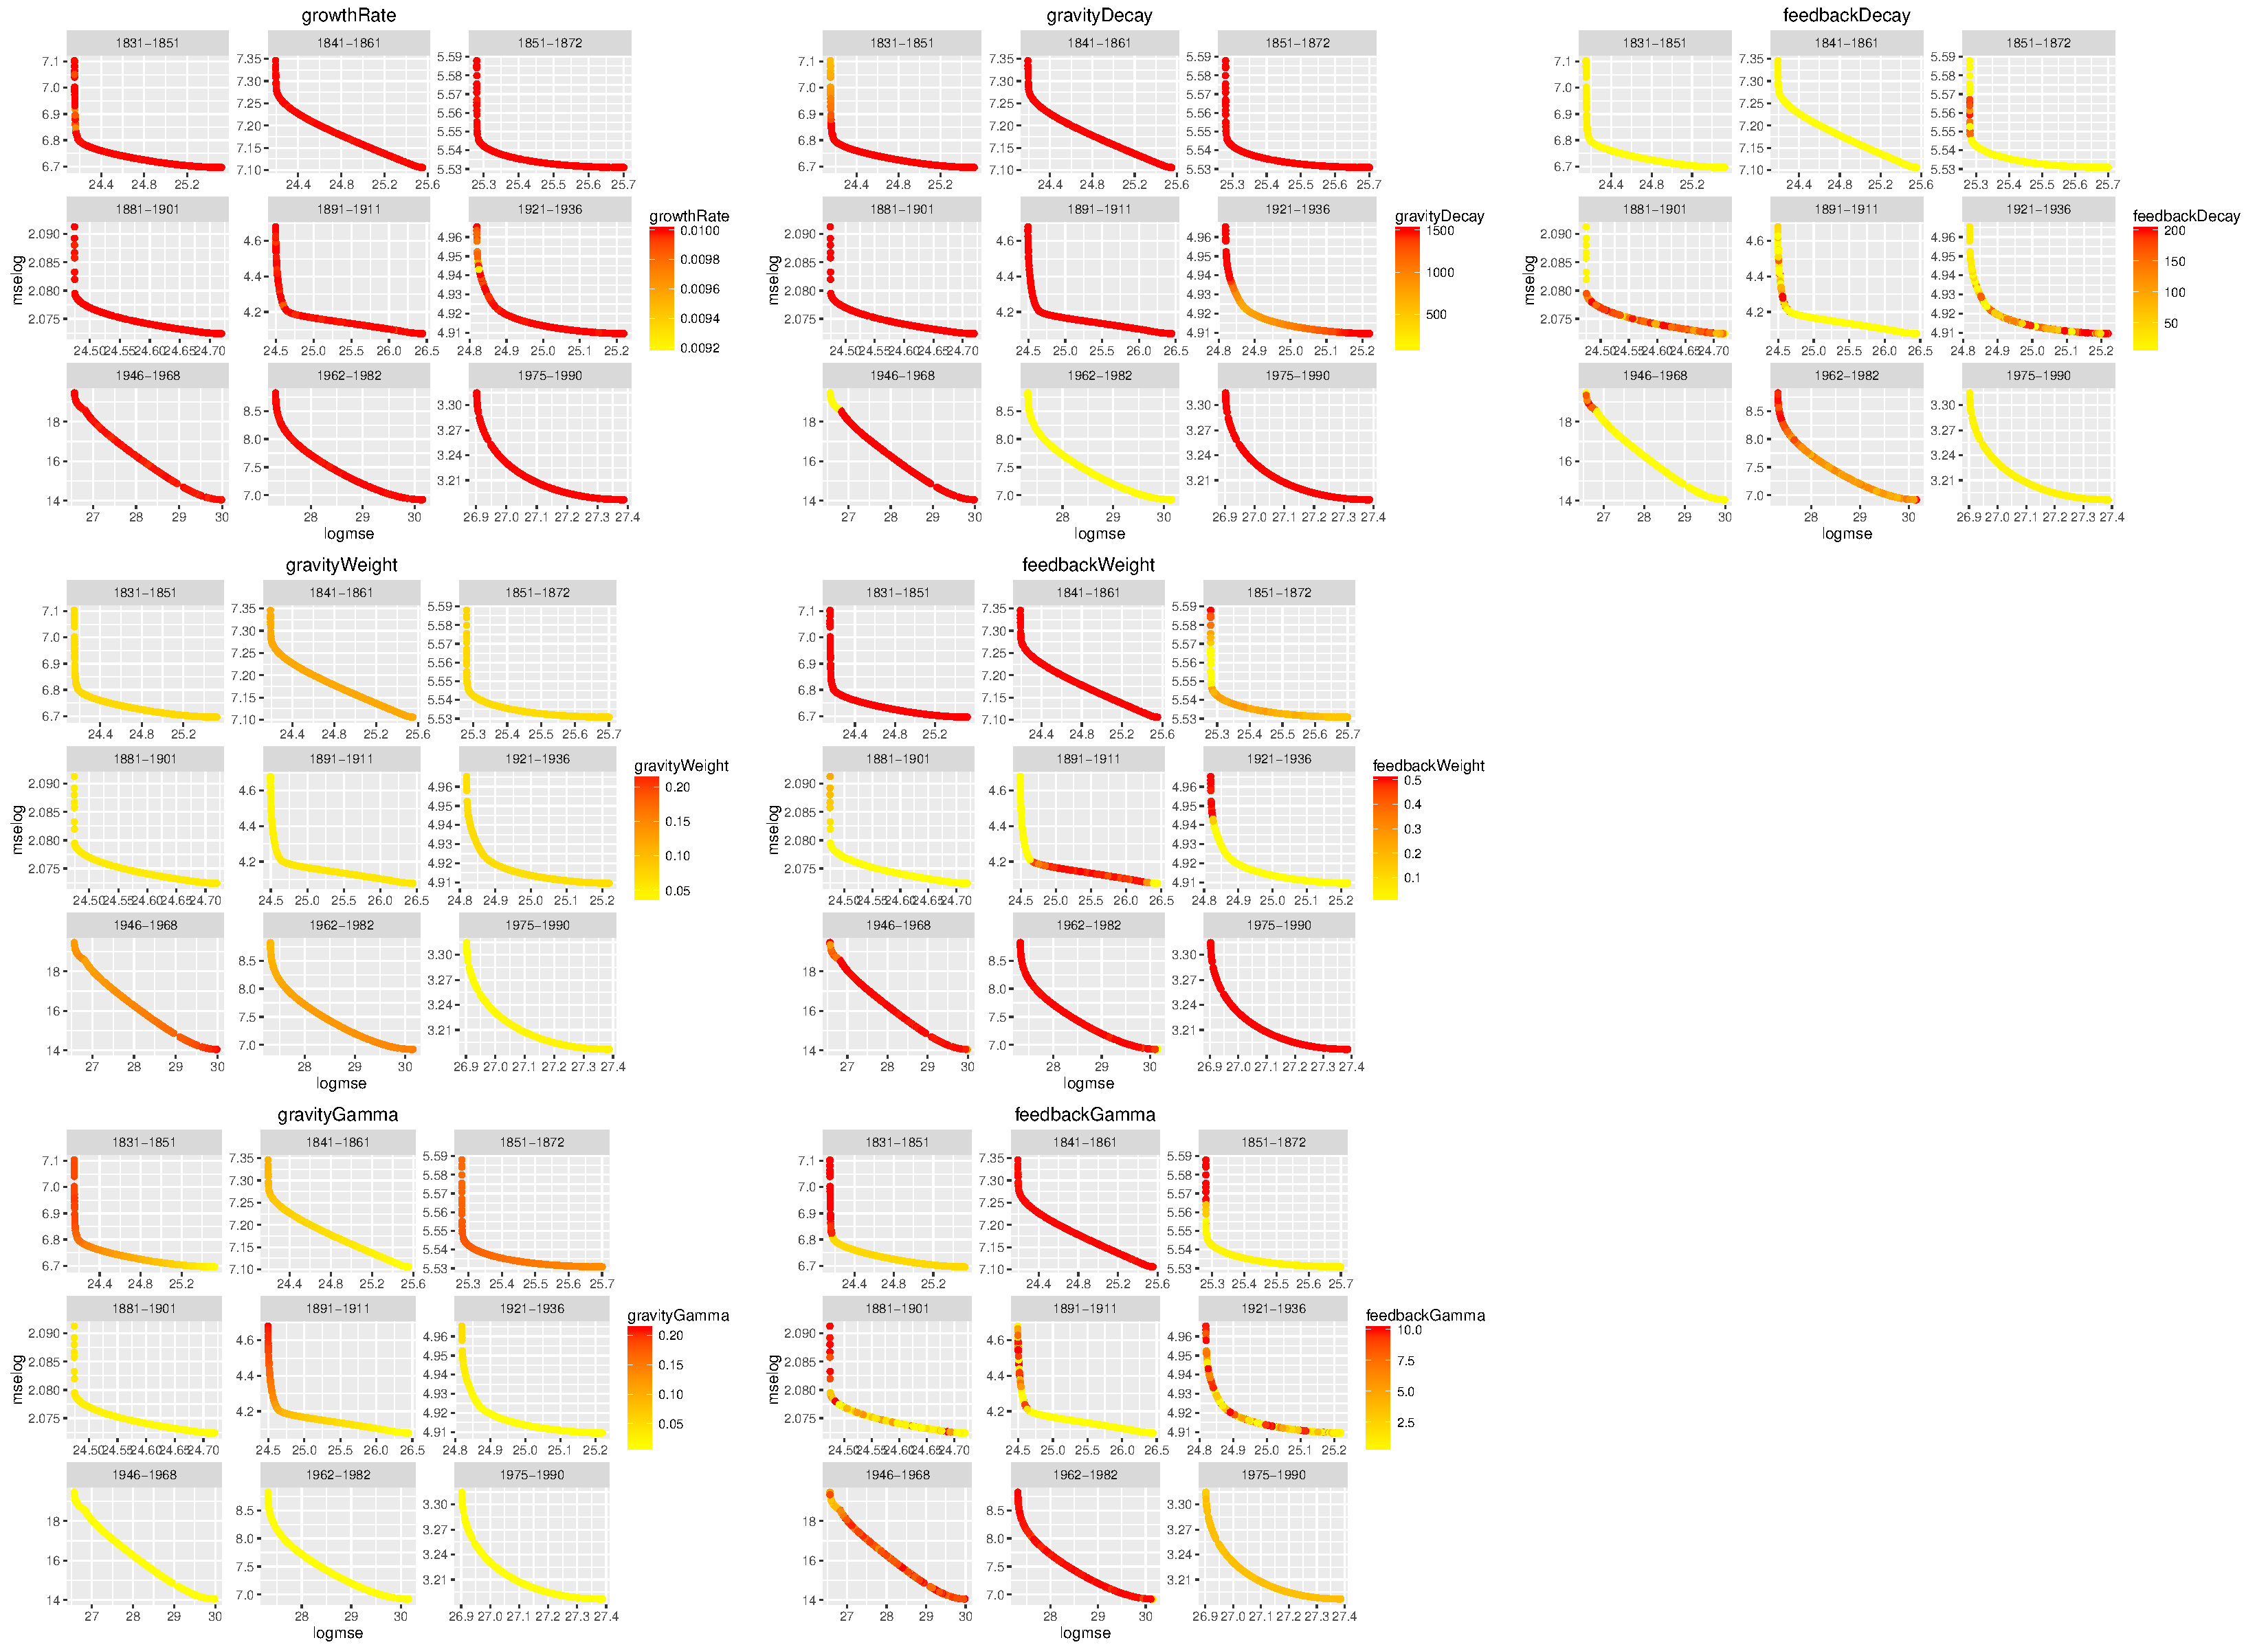
\includegraphics[width=\textwidth,height=0.8\textheight]{figures/allperiods_allparams}

}


\sframe{Quantifying overfitting : Empirical AIC}{

\justify

\vspace{-0.5cm}

\textit{Not clear nor well theorized how to deal with overfitting in models of simulation.} \textbf{Intuitive idea : } Approximate gain of information by approaching models of simulation by statistical models.

\medskip

Let $M_k^{\ast} = M_k\left[\alpha_k^{\ast}\right]$ computational models heuristically fitted to the same dataset. With $S_k \simeq M_k^{\ast}$, we show that $\Delta D_{KL}\left( M_k^{\ast},M_{k'}^{\ast}\right) \simeq \Delta D_{KL}\left( S_k,S_{k'}\right)$ if fits of $S_k$ are negligible compared to fit difference between computational models and models have same parameter number.

\bigskip

\textbf{Application} $M_1$ : gravity only model with $(r_0=0.0133,w_G=1.28e-4,\gamma_G=3.82,d_G=4e12)$ ; $M_2$ : full model with $(r_0=0.0128,w_G=1.30e-4,\gamma_G=3.80,d_G=8.4e14,w_N=0.603,\gamma_N=1.148,d_N=7.474)$

Fitting of independent polynomial models ($\tilde{P}_i(t) = Q\left[\tilde{P}_i(t-1)\right]$) with 4 and 7 parameters) gives $\Delta D_{KL} \simeq 19.7$ $\rightarrow$ fit improvement without overfitting


}





%%%%%%%%%%%%%%%%%
\section{Discussion}
%%%%%%%%%%%%%%%%%



\sframe{Discussion}{

\textbf{Theoretical and Methodological Implications}

$\rightarrow$ Indirect confirmation of known stylized facts (such as \textit{tunnel effect} through non-stationary calibration)

$\rightarrow$ For a better integration of theory, empirical and modeling on network aspects in evolutive urban theories 

$\rightarrow$ Methodology : first steps for empirical AIC in multi-modeling


\bigskip

\textbf{Further Developments}

$\rightarrow$ Need to validate the approach on other system/subsystem of cities~\cite{pumain2015multilevel}


$\rightarrow$ Add Real Network in a static/dynamic way : towards models of co-evolution of cities and network~\cite{raimbault2016memoire}


$\rightarrow$ Coupling with growth models at other level, as e.g. mesoscopic reaction-diffusion model~\cite{raimbault2016calibration}


}




\sframe{Conclusion}{

$\rightarrow$ Simple models of complex systems can have strong explanatory power, and be used to test hypothesis/confront a theory

\medskip

$\rightarrow$ Crucial role of interdisciplinarity and integration theory/empirical and qualitative/quantitative

%$\rightarrow$ interdisciplinarity as a way to transcend ``scientific cultural'' barriers

%\textbf{¡¡¡ bloody hell why are we not funding that ? !!! }


\bigskip
\bigskip
\bigskip


\footnotesize{ - All code and data available at \texttt{https://github.com/JusteRaimbault/CityNetwork/tree/master/Models\\
/NetworkNecessity/InteractionGibrat}

}

}




\sframe{Reserve slides}{

\centering

\Large

\textbf{Reserve Slides}

}




%%%%%%%%%%%%%%%%%%%%%
\begin{frame}[allowframebreaks]
\frametitle{References}
\bibliographystyle{apalike}
\bibliography{/Users/Juste/Documents/ComplexSystems/CityNetwork/Biblio/Bibtex/CityNetwork,biblio}
\end{frame}
%%%%%%%%%%%%%%%%%%%%%%%%%%%%




\sframe{Reserve slides}{

Calibration with fixed gravity effects (iterative calibration)

\centering

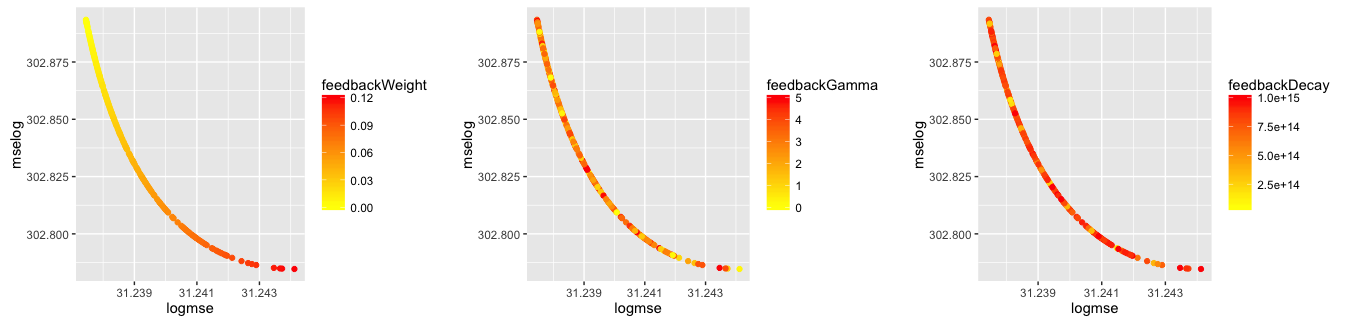
\includegraphics[width=\textwidth]{figures/pareto_gen213}

}









\end{document}







